\documentclass[aspectratio=169]{beamer}
\usetheme{Madrid}
\usecolortheme{beaver}
\usepackage[utf8]{inputenc}
\usepackage[T1]{fontenc}
\usepackage{tikz}
\usepackage{amssymb}
\usepackage{graphicx}
\setbeamertemplate{navigation symbols}{}
\setbeamercolor{title}{fg=white,bg=cyan!60!black}
\setbeamercolor{frametitle}{fg=white,bg=cyan!50!black}
\setbeamercolor{block title}{bg=cyan!15,fg=black}
\setbeamercolor{block body}{bg=cyan!5,fg=black}

\title{Block Arcade 3 — Events}
\subtitle{BOSS: Full Control}
\author{ByteForge --- Grade 7 --- Game Maker}
\date{}

\begin{document}

\begin{frame}
    \titlepage
\end{frame}

\begin{frame}{BOSS — four keys, four directions}
    \Large
    Each arrow key gets its OWN separate if — pressing two at once genuinely moves the sprite diagonally, for free.

    \begin{center}
    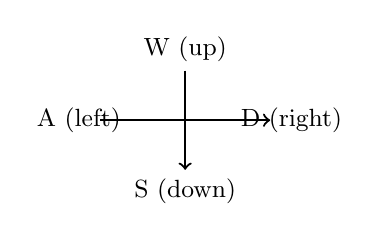
\begin{tikzpicture}[scale=0.9]

        \node at (0,0) {\small W (up)};
        \node at (0,-2) {\small S (down)};
        \node at (-1.5,-1) {\small A (left)};
        \node at (1.5,-1) {\small D (right)};
        \draw[->, thick] (0,-0.3) -- (0,-1.7);
        \draw[->, thick] (-1.2,-1) -- (1.2,-1);
        \node at (0,-1) {\small +};
    \end{tikzpicture}
    \end{center}
\end{frame}

\begin{frame}{Your Turn}
    \Large
    Open the student map, find \textbf{Block Arcade 3 — Events}, and complete
    the \textbf{BOSS} challenge --- everything you just saw, they now do themselves.
\end{frame}

\end{document}
